\chapter{Introduction}
This documentation contains information about the specifications, architecture, design and functionality of the electrically propulsed car dubbed 'AU2'. This system has been designed to be able to compete in Shell Eco Marathon (in the Prototype - Battery-electric category).

\begin{figure}[H]
	\centering
	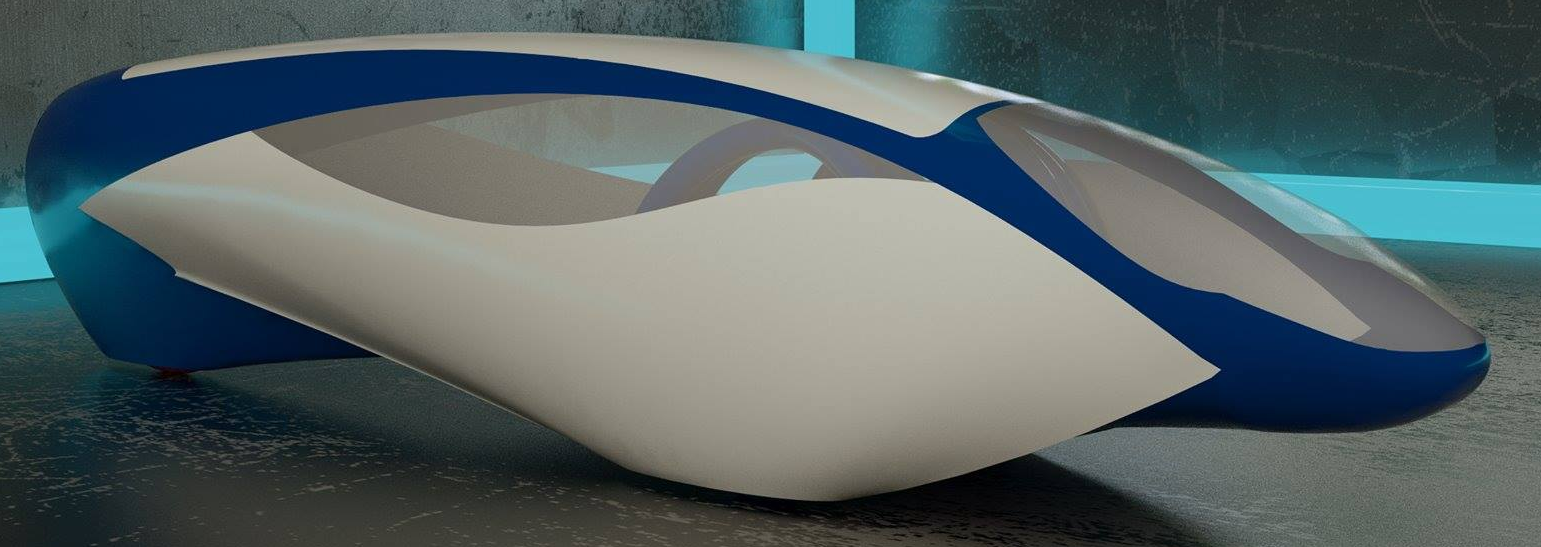
\includegraphics[width=0.6\linewidth]{Introduction/Model}
	\caption{Computer generated model of AU2}
	\label{fig:System_model}
\end{figure}

\section{System description}
The primary purpose of the car is to be as energy-effecient as possible, as this is the goal of Shell Eco Marathon. This is done by letting the car use an optimized driving algorithm. This algorithm is explained in greater details in later chapters. This algorithm can be turned on or off by the driver at the press of two buttons.

In order for the car to follow the technique's procedures correctly it has a variable energy-output to the electric motor. Furthermore, the car constantly measures the current speed and the amount of energy consumed. The measured parameters from a test-drive can be collected on a SD-card, if the user inserts such a card in the built-in SD-socket.

The car uses rechargable LiPo batteries which easily can be inserted/removed to allow a continuous driving experience. The battery is under constant surveillance by a Battery Management System (BMS) which measures the battery's energy-output and current temperature. This subsystem serves to protects the battery from overheating and protects the other circuits from an over-current.

As the car is designed to compete in Shell Eco-Marathon it must follow the safety procedures set down by Shell. This means that the car has a built-in safety mechanism. This mechanism consists of two switches: an on/off-switch and a dead man's switch. The dead man's switch must be pressed by the driver at all times in order for the car to drive. Lastly, the car contains an electrical horn which can be activated by the driver.

\begin{figure}[H]
	\centering
	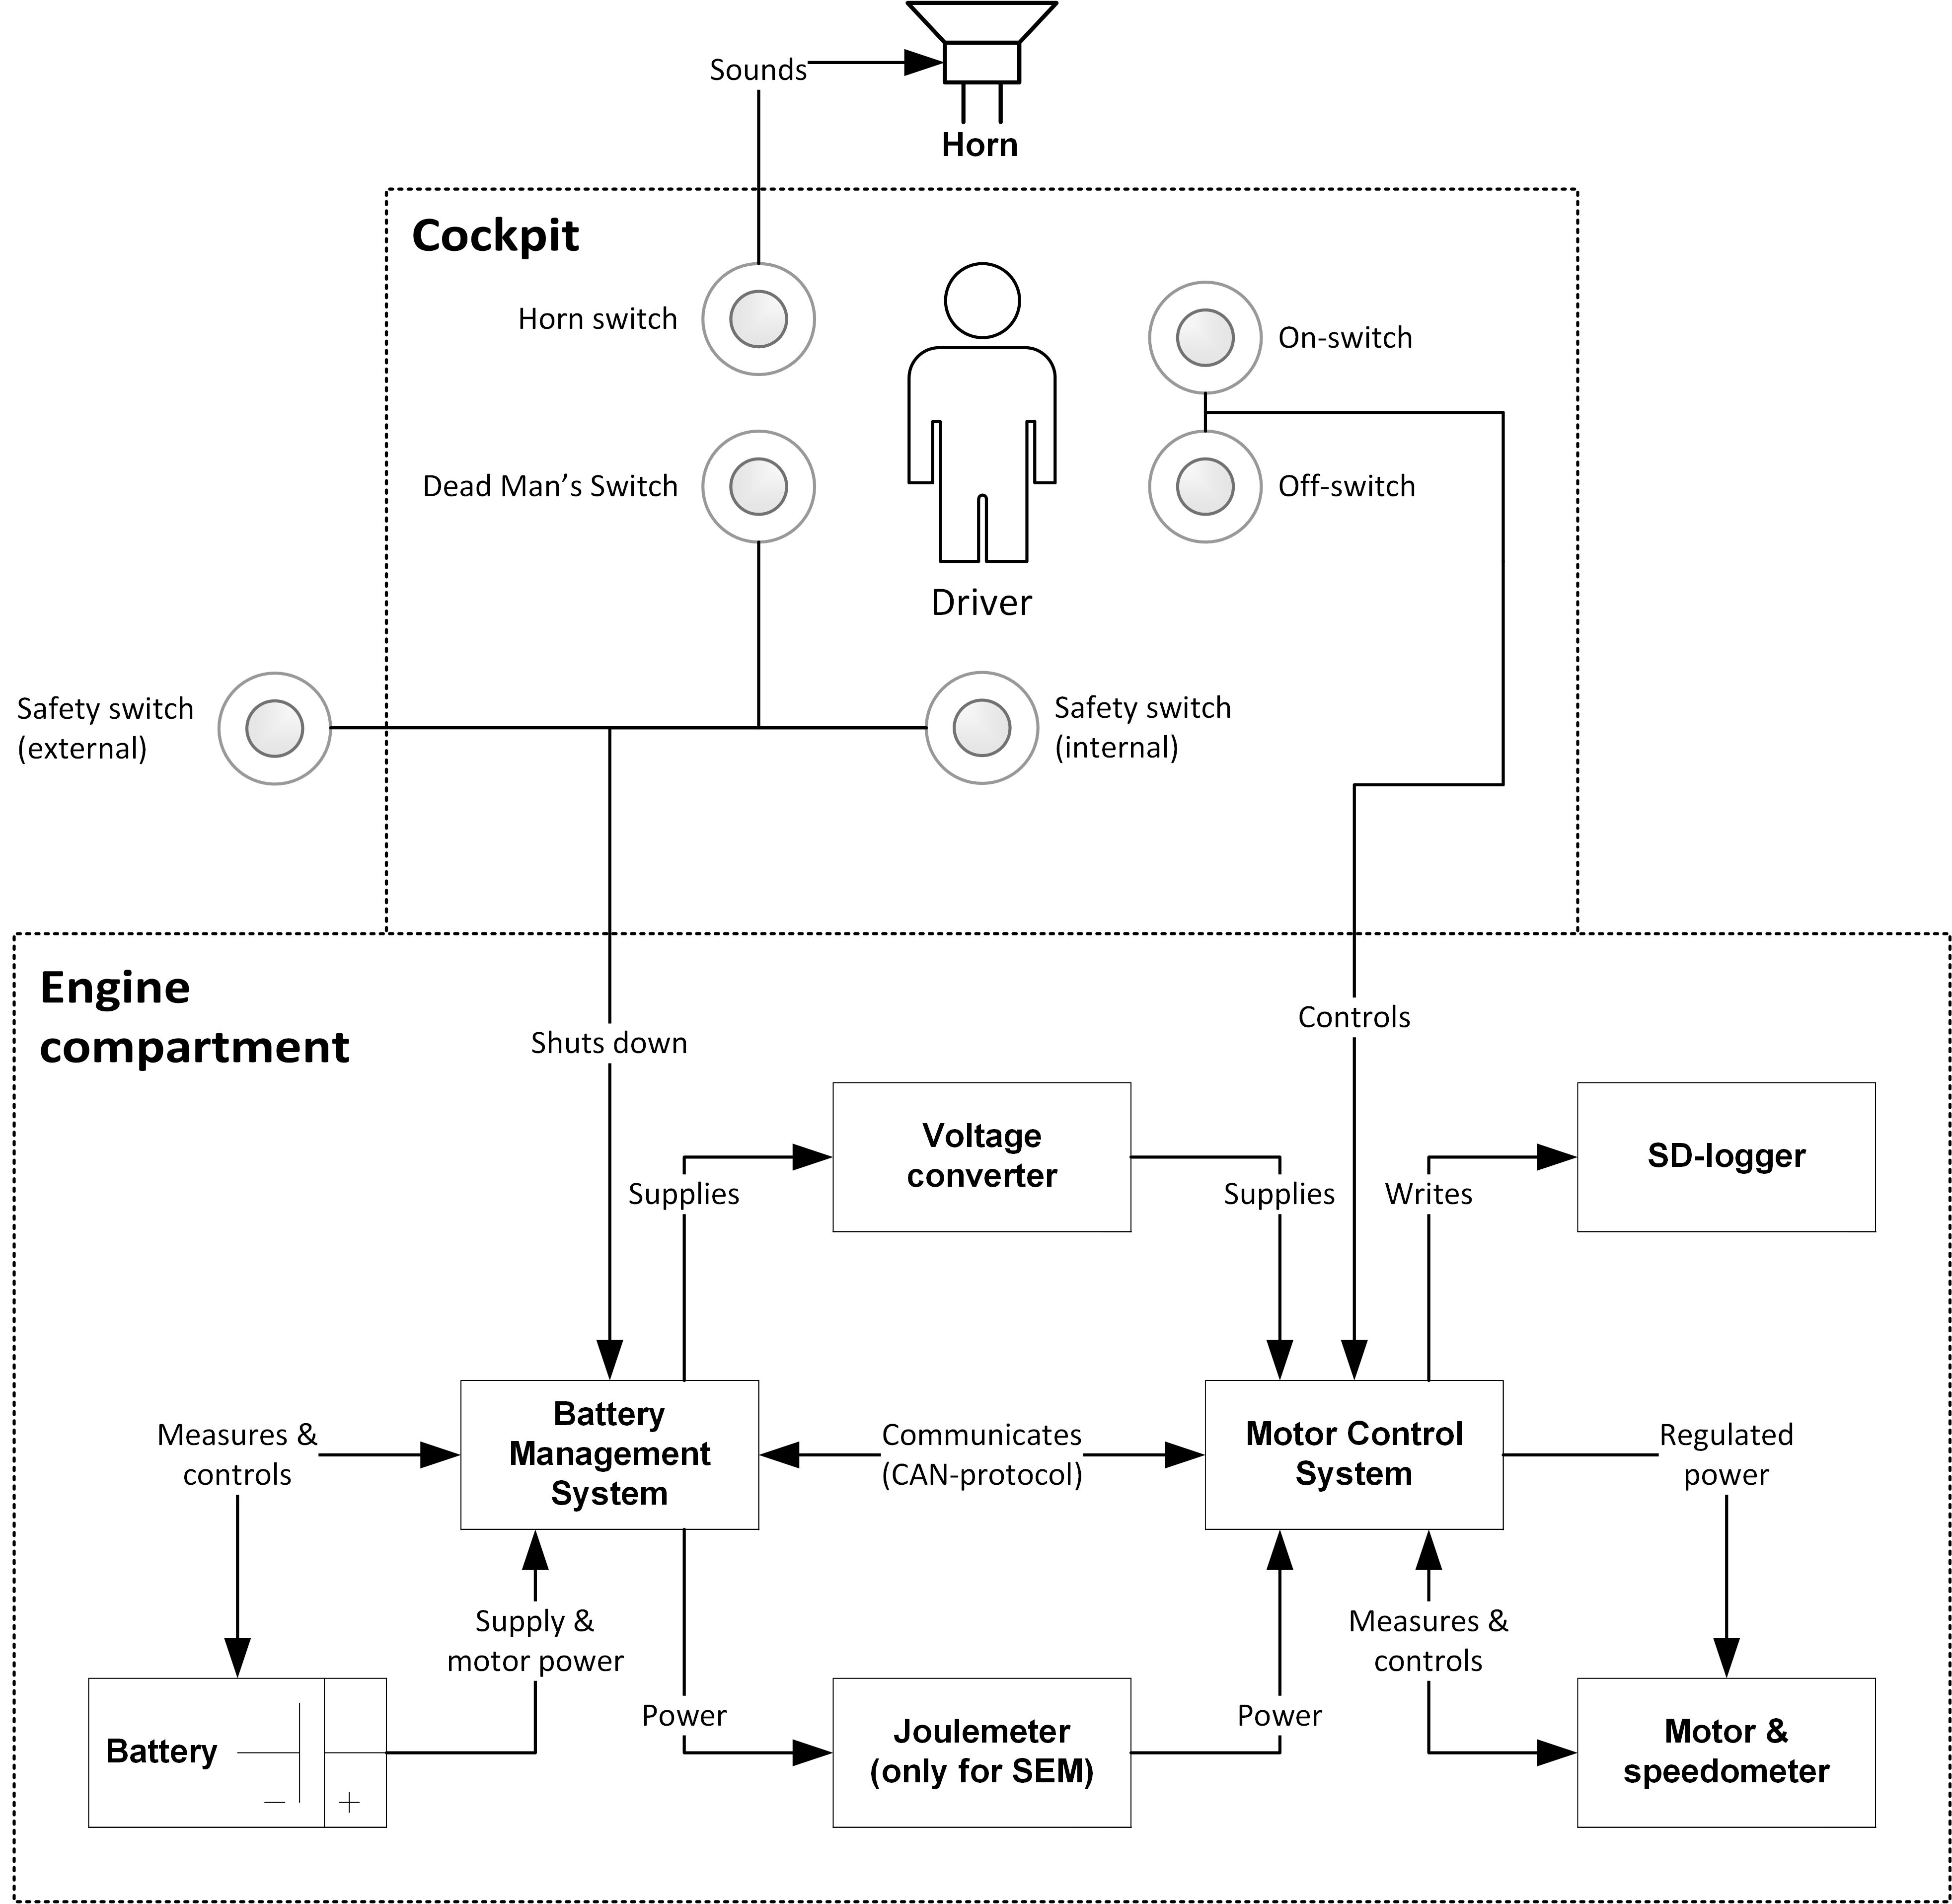
\includegraphics[width=1\linewidth]{Introduction/Overview}
	\caption{System overview}
	\label{fig:System_overview}
\end{figure}

\newpage
\section{List of terms}
The following list explains the various terms which have been used to refer to certain parts or subsystems in this documentation.

\begin{itemize}
	\item \textbf{SEM}\\
	Refers to Shell Eco Marathon which the car is designed to compete in.
	\item \textbf{Coast-and-burn}\\
	Refers to the driving algorithm which the car follows.
	\item \textbf{BMS}\\
	Refers to the Battery Management System which manages the output from the rechargable battery in order to protect the battery, as well as the other electrical systems in the car.
	\item \textbf{MCU}\\
	Refers to microprocessor being used in the project. MCU stands for Motor Controller Unit. The microprocessor chosen is a PSC 5LP Prototyping kit. It is build up around a Cortex M3. It is not to be confused with MCS which is the entire system for controlling the motor. 
	\item \textbf{PSoC}\\
	Refers to the CY8CKIT-059 PSoC 5LP Prototype Kit which is used as the Motorr Control Unit in the system.
	\item \textbf{Emergency Shutdown Switch}\\
	Refers to the Emergency System, which is a button that can be pressed. If pressed it triggers the BMS to disable all the power it supplies to the vehicle.
\end{itemize}